%! TeX root = thesis.tex
\chapter{Background}\label{background}
Here i will discuss background knowledge of Coverage Path Planning and surface curvature...

Things / topics i will cover:
\begin{enumerate}
	\item watershed segmentation... -> background, methodology
	\item UV Mapping -> background
	\item Geometry simplification -> methodology?
	\item Interior Edge Extension (and my modifications, if any) -> methodology
	\item boustrophedon -> methodology
	\item TSP -> background
	\item Modified TSP -> methodology
\end{enumerate}


\section{Geometric Curvature}
For segmenting a 3D mesh via Watershed Segmentation each vertex requires a singular / combined measure of curvature.
Various forms and types of curvature were examined throughout this project and are presented in the following sections.

\subsection{Principal Curvatures}
All combined measures of curvature are based, either in theory or in actuality, on the principal curvatures.
The principal curvatures at a given point on a surface are simply the maximum and minimum curvature\cite{DDGAppIntro_17_smooth_k}.
Determining principal curvatures for a continuous surface is unambiguous.
The principal curvatures of a surface $S$ at point $p$ are defined by the 2nd fundamental form\cite{DiffGeo_curves_surfaces, Basic_diff_geo_of_surfaces, DDGAppIntro_17_smooth_k}:
\begin{equation}
	II(X,Y) := \langle dN(X), df(Y)\rangle,
\end{equation}
and can be found as the eigenvalues of
\begin{equation}\label{2nd_fundamental_tensor}
	\begin{bmatrix}
		II(X_1, X_2) & II(X_1, X_2) \\
		II(X_2, X_1) & II(X_2, X_2)
	\end{bmatrix}.
\end{equation}
Similarly, the principal directions are the eigenvectors of \ref{2nd_fundamental_tensor}.

NOTE: maybe also include a graphic showing principal curvatures ?

There are however various ways of approximating the principal curvatures on a discrete mesh\cite{EstCurvOnTriMesh, DiscDiffGeoOpsTriMani}.
A basic approach is to calculate the mean and Gaussian curvatures, and derive the principal curvatures from them\cite{DDGAppIntro_19_discrete_k_2, Gauss_mean_k_notes}.
Given the mean curvature $H$ and Gaussian curvature $K$ (see \ref{sec:mean_k} and \ref{sec:gauss_k}), the principal curvatures can be calculated from \ref{eq:mean_k} and \ref{eq:gauss_k}.
\begin{align}
	\kappa_1 &= H - \sqrt{H^2 - K} \\
	\kappa_2 &= H + \sqrt{H^2 - K}
\end{align}
Although theoretically impossible, discretization errors can cause $H^2$ to be less than $K$, resulting in ``imaginary'' curvature.
This tends to occur on planar mesh regions, thus a minimum of 0 can be set for $H^2 - K$, because the root term would have been near 0 regardless, but it does highlight a flaw in this measure of curvature.

Taubin calculated the principal curvatures directly by estimating the tensor of curvature\cite{TaubinTensor}.
This has the benefit of direct calculation, but has been shown to be succeptible to noise in the mesh\cite{Comp_k_notes}.
Thiesel et al. calculate the curvature tensor per triangular face in the mesh, based on the face's corner normals\cite{Norm_based_k_tensor_est}.
Rusinkiewicz took a slightly different approach, calculating the curvature tensor for each mesh face via the differences between corner normals\cite{SRTensor}.
From there he computes the per vertex curvature tensor as a weighted sum over the curvature tensors of the vertex's adjoining triangles via coordinate system transformations.
Gatzke and Grimm examine a variety of other curvature estimation methods\cite{EstCurvOnTriMesh}, most of which were not considered for this work.

\subsection{Mean Curvature}\label{sec:mean_k}
Mean curvature is, as the name implies, the mean of the principal curvatures\cite{DDGAppIntro_19_discrete_k_2}:
\begin{equation}\label{eq:mean_k}
	H = \frac{\kappa_1 + \kappa_2}{2}
\end{equation}
Mean curvature can be approximated on a discrete mesh via edge angle product sum:
\begin{equation}
	H := \frac{1}{2}\sum_{i j \in E}l_{ij} \phi_{ij}
\end{equation}.
Alternatively, the mean curvature can be calculated via the discrete Laplace-Beltrami operator:
\begin{equation}
	H := \frac{1}{2}\sum_{i j \in E}(\cot \alpha_{ij} + \cot \beta_{ij})(f_j - f_i).
\end{equation}

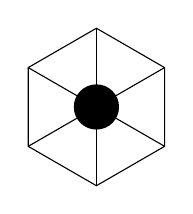
\begin{tikzpicture}[vertex/.style={circle,fill=black}]
	\newdimen\R
	\R=1cm
	\node[vertex] (0, 0) {i};
	\draw (330: \R) \foreach \x in {30,90,...,330} { -- (\x:\R) };
	\foreach \x in {30,90,...,330} {
		\draw (0, 0) -- (\x:\R);
		\draw [vertex] (\x:\R);
	}
\end{tikzpicture}
\includegraphics[width=0.3\textwidth]{../resources/ddg_disc_k_1_mean_k.png}

\subsection{Gaussian Curvature}\label{sec:gauss_k}
Gaussian curvature\cite{TheoremaEgregium} is the product of the principal curvatures:

\begin{equation}\label{eq:gauss_k}
	K = \kappa_1 * \kappa_2
\end{equation}

The discrete Gaussian curvature at a vertex is typically approximated as the ``angle defect'' divided by the vertex's area:
\begin{equation}
	K = \frac{2\pi - \sum \Theta_j}{A_i}.
\end{equation}

Image comparing mean and gaussian curvature

\subsection{Root Mean Square Curvature}
Pulla et al. propsed using the root mean square curvature as the curvature estimate for use during watershed segmentation:
\begin{equation}
	\kappa_{rms} = \sqrt{\frac{\kappa_1^2 + \kappa_2^2}{2}}.
\end{equation}
They compared different measures of curvature for this purpose and found that it was approximately as good as absolute curvature:
\begin{equation}
	\kappa_{abs} = |\kappa_1| + |\kappa_2|,
\end{equation}
but cheaper to compute, because they computed $\kappa_{rms}$ from the mean and Gaussian curvatures using:
\begin{equation}
	\kappa_{rms} = \sqrt{4H^2 - 2K}.
\end{equation}

\subsection{Derivative of Curvature}
Through testing it was determined that supplying the derivative of curvature instead of the curvature itself to watershed segmentation would better preserve the boundaries between semantic regions.
Rusinkiewicz proposes a method of taking the derivative of the curvature tensor\cite{SRTensor}.
Because watershed segmentation expects a single value rather than a tensor, the magnitude of the derivative of the curvature tensor was approximated as the sum of squares of said tensor.

\section{UV Mapping}
UV Mapping is the process of projecting a surface from 3D to 2D, effectively ``unwrapping'' the 3D surface.
(insert sentence about common usage in 3D modeling / graphics and textures)
The UV map for planar surfaces is trivial, as the 3D surface is already ``unwrapped''.

\subsection{Conic Surfaces}
General equation of a conic is:
\begin{equation}\label{eq:gen_conic}
	Ax^2 + Bxy + Cy^2 + Dx + Ey + F = 0
\end{equation}

\subsubsection{Elliptic Surface}
General equation:
\begin{equation}
	\frac{x^2}{a^2} + \frac{y^2}{b^2} = 1
\end{equation}
To obtain a vector perpendicular to a point on the ellipse, the derivative of said point is rotated 90 degrees.
The point, as a function of the angle $\theta$:
\begin{equation}
	(x,y) = (a\cos\theta, b\sin\theta)
\end{equation}
The derivative thereof:
\begin{equation}
	\frac{d}{d\theta}(x,y) = (-a\sin\theta, b\cos\theta)
\end{equation}
Rotated -90 degrees:
\begin{equation}
	\text{Rot}_{90}\frac{d}{d\theta}(x,y) = (b\cos\theta, a\sin\theta)
\end{equation}

\subsubsection{Parabolic Surface}
Parabolas are much simpler than and ellipses and hyperbolas, as can be seen by the following equations.
The parametric general equation of a parabola is:
\begin{equation}
	-\sin\theta x + \cos\theta y = \frac{1}{4f}(\cos\theta x + \sin\theta y - h)^2 + k
\end{equation}
To solve for the conic parameters of a parabola the general equation's quadratic term is expanded and like terms gathered:
\begin{multline*}
	-\sin\theta x + \cos\theta y = \frac{1}{4f}(\cos^2\theta x^2 + \cos\theta\sin\theta xy \\
	- h \cos\theta x + \cos\theta\sin\theta xy + \sin^2\theta y^2 - h\sin\theta y - h \cos\theta x - h \sin\theta y + h^2) + k
\end{multline*}
\begin{multline*}
	\frac{\cos^2\theta}{4f} x^2 + \frac{2\cos\theta\sin\theta}{4f} xy + \frac{\sin^2\theta}{4f} y^2 \\
	+ \left(\sin\theta - \frac{2h \cos\theta}{4f}\right)x + \left(\cos\theta - \frac{2h \sin\theta}{4f}\right)y + \frac{h^2}{4f} + k = 0
\end{multline*}
\begin{align}
	A &= \frac{\cos^2\theta}{4f} \\
	B &= \frac{2\cos\theta\sin\theta}{4f} \\
	C &= \frac{\sin^2\theta}{4f} \\
	D &= \sin\theta - \frac{2h \cos\theta}{4f} \\
	E &= \cos\theta - \frac{2h \sin\theta}{4f} \\
	F &= \frac{h^2}{4f} + k
\end{align}

\subsubsection{Hyperbolic Surface}
\begin{equation}
\begin{split}
	\frac{(\cos\theta(x-h) + \sin\theta(y-k))^2}{a^2} - \frac{(\cos\theta(y-k) + \sin\theta(x-h))^2}{b^2} &= 1 \\
	\frac{(x_c + y_s)^2}{a^2} - \frac{(y_c + x_s)^2}{b^2} &= 1 \\
	b^2(x_c^2 + 2x_c y_s + y_s^2) - a^2(y_c^2 + 2 x_s y_c + x_s^2) &= a^2 b^2 \\
	b^2 x_c^2 + 2 b^2 x_c y_s + b^2 y_s^2 - a^2 y_c^2 - 2 a^2 x_s y_c - a^2 x_s^2 - a^2 b^2 &= 0 \\
	b^2 x_c^2 - a^2 x_s^2 + 2 b^2 x_c y_s - 2 a^2 x_s y_c + b^2 y_s^2 - a^2 y_c^2 - a^2 b^2 &= 0 \\
\end{split}
\end{equation}
\begin{multline*}
	b^2 (\cos\theta(x-h))^2 - a^2 (\sin\theta(x-h))^2 \\
	+ 2 b^2 \cos\theta(x-h) \sin\theta(y-k) - 2 a^2 \sin\theta(x-h) \cos\theta(y-k) \\
	+ b^2 (\sin\theta(y-k))^2 - a^2 (\cos\theta(y-k))^2 - a^2 b^2 = 0
\end{multline*}
\begin{multline*}
	(b^2 \cos^2\theta - a^2 \sin^2\theta)(x-h)^2 \\
	+ 2 \cos\theta\sin\theta(b^2 - a^2)(x-h)(y-k) \\
	+ (b^2 \sin^2\theta - a^2 \cos^2\theta)(y-k)^2 - a^2 b^2 = 0
\end{multline*}
\begin{equation*}
	\begin{split}
		c_1(x-h)^2 + c_2(x-h)(y-k) + c_3(y-k)^2 - a^2 b^2 &= 0 \\
		c_1(x^2-2hx + h^2) + c_2(xy-hy-kx+hk) + c_3(y^2-2ky+k^2) - a^2 b^2 &= 0 \\
		c_1 x^2 + c_2 xy + c_3 y^2 + (-2h c_1 -k c_2) x + (-h c_2 -2k c_3)y + c_1 h^2 + c_2 hk + c_3 k^2 - a^2 b^2 &= 0 \\
	\end{split}
\end{equation*}
\begin{align*}
	A &= c_1 = b^2 \cos^2\theta - a^2 \sin^2\theta \\
	B &= c_2 = 2 \cos\theta\sin\theta(b^2 - a^2) \\
	C &= c_3 = b^2 \sin^2\theta - a^2 \cos^2\theta \\
	D &= (-2h c_1 -k c_2) \\
	E &= (-h c_2 -2k c_3) \\
	F &= c_1 h^2 + c_2 hk + c_3 k^2 - a^2 b^2
\end{align*}
Now to solve for $a$, $b$, and $\theta$:
Solving $A$ for $b^2$:
\begin{equation}
	\begin{split}
		A &= b^2 \cos^2\theta - a^2 \sin^2\theta \\
		b^2 &= \frac{A}{\cos^2\theta} + a^2\tan^2\theta \\
	\end{split}
\end{equation}
Setting 3.6 into $C$ and solving for $a^2$:
\begin{equation}
	\begin{split}
		C &= b^2 \sin^2\theta - a^2 \cos^2\theta \\
		a^2 &= -\frac{C}{\cos^2\theta} + b^2\tan^2\theta \\
		a^2 &= -\frac{C}{\cos^2\theta} + \left(\frac{A}{\cos^2\theta} + a^2\tan^2\theta\right)\tan^2\theta \\
		\cos^4\theta a^2 &= -C\cos^2\theta + A\cos^2\theta + \sin^4\theta a^2 \\
		(\cos^4\theta - \sin^4\theta) a^2  &= \cos^2\theta(A-C) \\
		a^2  &= \frac{\cos^2\theta(A-C)}{(\cos^4\theta - \sin^4\theta)} \\
	\end{split}
\end{equation}
Setting 3.6 into $B$:
\begin{equation}
	\begin{split}
		B &= 2 \cos\theta\sin\theta(\frac{A}{\cos^2\theta} + a^2\tan^2\theta - a^2) \\
		\cos^2\theta B &= 2 \cos\theta\sin\theta(A + (\sin^2\theta - \cos^2\theta) a^2) \\
	\end{split}
\end{equation}
Setting 3.7 into 3.8:
\begin{equation}
	\begin{split}
		\cos^2\theta B &= 2 \cos\theta\sin\theta(A + (\sin^2\theta - \cos^2\theta) \frac{\cos^2\theta(A-C)}{(\cos^4\theta - \sin^4\theta)}) \\
	\end{split}
\end{equation}

\section{Traveling Salesman Problem}


